\chapter{Introduction}
\label{chap:introduction}
\section{Motivation} 
\label{sec:motivation}
In the domain of computational finance, much research is performed to find and improve algorithms that help maximize revenue. Among other things, this may be achieved through profitable trades or through minimization of inevitably occurring costs. In most exchange markets, asset prices are determined by supply and demand: While large demand for an asset results in higher prices, oversupply has the opposite effect of lowering prices. A \emph{fair} price is automatically derived from the universe of opposing trading interests.\\

This observation is consolidated in Fama's \emph{efficient market hypothesis}\Cite{Fama70efficientcapital}, which assumes markets to be extremely \emph{efficient}. In efficient markets news are assumed to spread so fast, that all relevant informations are incorporated into the respective assets price instantaneously and unimpeded. Future price changes reflect only future news and are independent of todays price changes. Consequently, as news are per definition unpredictable, future price changes are unpredictable and random. According to this theory, it should neither be possible for investors to earn above average returns from the overall market by purchasing undervalued shares and selling shares for inflated prices, nor to profit from proper order placement deliberately.\\

In \Cite{TheEfficentMarketHypothesisAndItsCritics} Malkiel shows empirically and theoretically that the efficient market hypothesis is only valid under certain preconditions. While the paper concludes that stock markets are far less predictable than some (at that time) recent academic papers claimed, there remains a certain degree at which asset prices are indeed predictable.\\

Investors participating in exchange markets must expect fees, charged by the respective market place organizer in return for granting access to their infrastructure. Other than that, there are hidden costs to be considered as well: While trades involving little capital\footnote{Little capital, relative to the whole market liquidity.} usually cause minor impact on the current market situation, large-scale investors must be cautious when it comes to order placements. Large orders can have a major impact on supply and demand, leading to diminishing availability and consequently \emph{hidden costs} in form of worsening prices.\\

While direct costs are contractually regulated and thus predictable to a large extend, this is not the case for hidden costs. The unpredictable nature of hidden costs bears a significant risk that grows exponentially with the trading volume pursued. This motivates for well considered trading strategies, that help to reduce the investors impact and avoid causing costly market turbulences by unwinding large orders of shares over time.



\section{Objectives}
\label{sec:objectives}
Most trading strategies deal with a large diversified portfolio to reduce risk. Past stock prices are studied in an attempt to predict future prices and to decide on which assets to buy and which to sell.\\

This thesis tackles the important problem of \emph{optimized trade execution}, which aims to obtain the best possible price for a trade instructed by higher level investment decisions. \Cref{fig:optimizedtradeexecution} shows exemplary how optimized trade execution \\



In its simplest form, the problem is defined by a particular financial instrument (here: bitcoins), which must be bought or sold within a fixed time horizon, while minimizing the expenditure (share price) for doing so.\\

\begin{figure}[ht]
	\centering
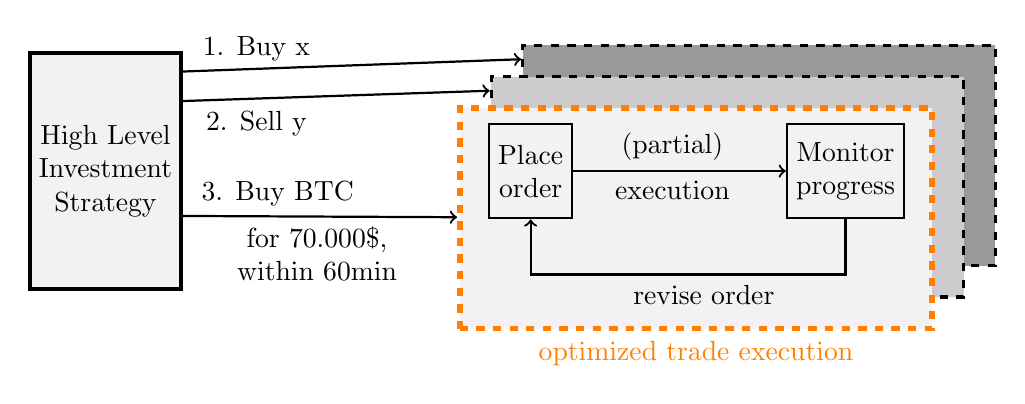
\begin{tikzpicture}[node distance = 16em, auto, thick]
    \node[draw, minimum height=3cm, align=center, fill=black!5, line width=0.5mm] at (0, 0)   (A) {High Level\\Investment\\Strategy};
    \node[draw, black, dashed, minimum height=2.8cm, minimum width=6cm, line width=0.4mm, fill=black!40] at (8.3,0.2) (X2) {};
    \draw[->] (A.52) node[above, xshift=2.7cm] {}  node[above, align=center, xshift=0.93cm]{1. Buy x}  -- (X2.158);
    
    \node[draw, black, dashed, minimum height=2.8cm, minimum width=6cm, line width=0.4mm, fill=black!20] at (7.9,-0.2) (X1) {};
    \draw[->] (A.42) node[above, xshift=2.7cm] {}  node[below, align=center, xshift=0.93cm]{2. Sell y} -- (X1.158);

    \node[draw, orange, dashed, minimum height=2.8cm, minimum width=6cm, line width=0.7mm, fill=black!5, label={below, orange: optimized trade execution}] at (7.5,-0.6) (X) {}; 
%    \draw[->] (A) node[above, xshift=2.7cm] {}  node[below, align=center, xshift=2.7cm]{Sell x} -- (X1);

%    \node[draw, minimum height=2.8cm,minimum width=5cm, label={below: optimized trade execution}] {xx} ;


    

    \node[draw, minimum height=1.2cm, align=center] at (5.4, 0)   (B) {Place\\order};
    \node[draw, minimum height=1.2cm, align=center] at (9.4, 0)   (C) {Monitor\\progress};
%    \node[draw, minimum height=1.2cm, align=center] at (11, 0)   (D) {done};
%    \node[draw] at (12, 0)   (E) {Application};

    
    \draw[->] (A.-30) node[above, xshift=1.2cm] {3. Buy BTC}  node[below, align=center, xshift=1.7cm]{for $70.000\$$,\\within 60min} -- (X);

    \draw[->] (C.south) node[below, xshift=-1.8cm, yshift=-0.7cm] {revise order}  -- ++(-0,0) -- ++(0,-0.7) -| (B);

    \draw[->] (B) node[above, xshift=1.8cm] {(partial)} node[below, xshift=1.8cm] {execution}  -- (C);

%    \draw[->] (C) node[above, xshift=2.1cm] {}  -- (D);

\end{tikzpicture}
	\caption{Optimized Trade Execution.}
	\label{fig:optimizedtradeexecution}
\end{figure}

The scope of this thesis is to transfer Nevmyvakas \cite{Nevmyvaka:2006} reinforcement learning approach from traditional stock markets with expensive, proprietary data sources, to the relatively young market of bitcoin trading and to improve it's general ability to solve the important problem of optimized trade execution. In contrast to their experiments this thesis builds on inexpensive, publicly retrievable bitcoin exchange data. Snapshots of the current market situation are retrieved on a low-resolution, minute-scale basis from the open bitcoin exchange platform Poloniex. As such the usability of the retrieved dataset remains to be shown. \\

Additional market features, describing the current market situation as well as historic market performance, are evaluated in terms of cost impact. An Orderbook Trading Simulator (OTS), which simulates the individual traders influence on the current market situation, is implemented and used in order to learn and evaluate various trading strategies.


\section{Related Work}
\label{sec:relatedwork}
x

\section{Contributions}
\label{sec:contributions}
\begin{itemize}
\item An orderbook trading simulator framework is presented which takes into account the individual traders influence on the current market situation.

\end{itemize}

\section{Outline of Contents}
\label{sec:outline}
The remainder of this thesis is structured as follows:\\
\Cref{chap:background} gives a general introduction into the vocabulary of financial computing and the machine learning techniques employed, \Cref{chap:simulator} describes the Orderbook Trading  Simulator, developed within the scope of this thesis, and \Cref{chap:reinforcementlearning} covers the machine learning part. \Cref{chap:conclusion} closes with a conclusion and discussion.


\cleardoublepage{}